%%%% ijcai11.tex

\typeout{Semi-supervised structuring of complex data}

% These are the instructions for authors for IJCAI-13.
% They are the same as the ones for IJCAI-11 with superficical wording
%   changes only.

\documentclass{article}
% The file ijcai13.sty is the style file for IJCAI-13 (same as ijcai07.sty).
\usepackage{ijcai13}

% Use the postscript times font!
\usepackage{times}
\usepackage[pdftex]{graphicx}
\DeclareGraphicsExtensions{.pdf}
%\usepackage{hyperref}

\pdfinfo{
/Title (Semi-supervised structuring of complex data)
/Subject (Extended abstract of the PhD thesis of Marian-Andrei Rizoiu)
/Author (Marian-Andrei Rizoiu)
/Keywords (pdh thesis, semi-supervised clustering, complex data, temporal clustering, data representation, research, data mining, machine learning)
}

%\hypersetup
%{
%pdftitle={},%
%pdfauthor={},%
%pdfsubject={}%
%}

\title{Semi-supervised
structuring of complex data\thanks{PhD prepared under the supervision of St\'ephane Lallich and Julien Velcin, professors at the University Lumi\`ere Lyon 2.}}

\author{Marian-Andrei Rizoiu \\
ERIC Laboratory \\
University Lumi\`ere Lyon 2 \\
Lyon, France \\
Marian-Andrei.Rizoiu@univ-lyon2.fr}

\begin{document}

\maketitle

\begin{abstract}
The objective of the thesis is to explore how complex data can be treated using unsupervised machine learning techniques, in which additional information is injected to guide the exploratory process.
Starting from specific problems, our contributions take into account the different dimensions of the complex data: their nature (image, text), the additional information attached to the data (labels, structure, concept ontologies) and the temporal dimension.
A special attention is given to data representation and how additional information can be leveraged to improve this representation.
\end{abstract}

\section{The big picture}

The general context of the research in this thesis lies at the intersection of \textbf{Complex Data Analysis} and \textbf{Semi-Supervised Clustering}.
The research project behind the thesis was built incrementally through a dialectical relation between theory and practice.
The research projects in which I was involved raised several precise problems, which usually dealt with handling complex data (heterogeneous data of different natures, \textit{e.g.}, text, image) and embedding additional information into the learning process.

The different contributions of the thesis can be structured conceptually as show in Figure~\ref{fig:streamlined-schema}.
The center points are translating data of different natures into a representation format understandable by machine learning algorithms and knowledge injection into the unsupervised learning algorithms and data representation constructors.

\subsection{Dealing with Complex Data}
\label{subsec:complex-data}

\begin{figure}[!t]
	\centering
	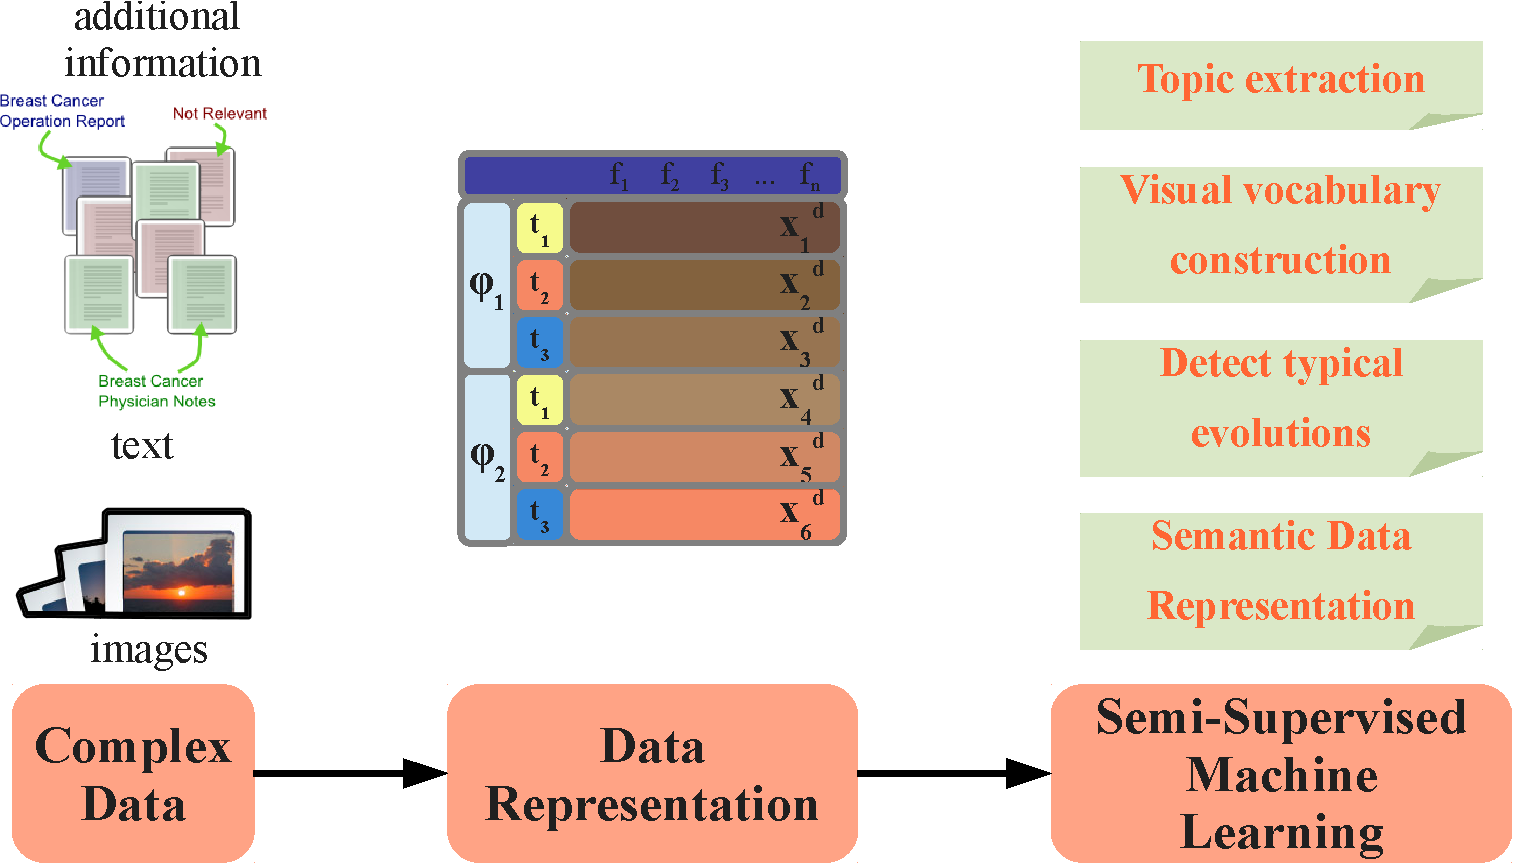
\includegraphics[width=0.48\textwidth]{streamlined-schema}
	
	\caption{Conceptual organization of the work in the thesis.}
	\label{fig:streamlined-schema}
\end{figure}

Complex Data is difficult to process efficiently~\cite{ZIG09}.
Its nature can be very diverse (\textit{i.e.}, text, image or audio/video data).
It is heterogeneous, as it may come from multiple sources.
It is often temporal, as the evolution of different entities is recorded through time.
Also, additional information and knowledge is attached to the data, under the form of user labels, structure of interconnected documents or knowledge bases.

A straightforward method for dealing with complex data of different natures is to transform them into a tabular numerical format and to apply classical Machine Learning algorithms.
Most Data Mining algorithms were developed to use data in this format.
The tabular format is a simple way to describe an instance as a measurement vector on a set of predefined features.
Today's challenges lie in rendering the data into a common usable numeric format which succeeds in capturing the information present in the native format, and in efficiently using external information for both creating the format and improving the results of analysis.

\subsection{Semi-supervised Clustering}

Leveraging partial expert knowledge into clustering represents the domain of semi-supervised clustering.
Unlike semi-supervised learning, where the accent is on dealing with missing data in supervised algorithms, semi-supervised clustering is used when the expert knowledge is in such low quantity that is would be impossible to apply supervised techniques.
The expert knowledge is under the form of either class labels, or pairwise constraints,
%~\cite{WAG01}
and it is used to guide the clustering process in the solutions space.
%Pairwise constraints are either ``must-link'' (the observations must be placed in the same cluster) or ``cannot-link'' (the two observations cannot be placed in the same cluster).
%Depending on the method in which supervision is introduced into clustering, \cite{GRI05} divides the semi-supervised clustering methods into two classes:
%a) the similarity-adapting methods~\cite{BIL03,COH03,KLE02,XIN02}, which seek to learn new similarity measures in order to satisfy the constraints, and 
%b) the search-based methods~\cite{WAG01,BAS02,DEM99} in which the clustering algorithm itself is modified.
Both the additional information that comes with the complex data and its temporal component can be modeled using semi-supervised clustering techniques.

\section{Contributions}

\paragraph{Detecting Typical Evolutions}
One of our driving interests is how to leverage the temporal information into clustering.
In ~\cite{RIZ12}, we detect typical evolutions of entities by proposing a new temporal-aware dissimilarity measure and a segmentation contiguity penalty function. 
We combine the spatio-temporal dimension of complex data with a semi-supervised clustering technique. 
We propose a novel time-driven constrained clustering algorithm, called TDCK-Means, which creates a partition of coherent clusters, both in the multidimensional space and in the temporal space.
We improve TDCK-Means in~\cite{RIZ13c} by adding the possibility to fube tune the impact of the temporal-component and to structure the detected evolutions as a cluster graph.

\paragraph{Using Data Semantics to Improve Data Representation}
As Section~\ref{subsec:complex-data} shows, treating data of different types (image, text) usually boils down to rendering the data into a Tabular Numeric Format and applying classical Machine Learning algorithms.
We give a special importance to improving representation of the data in this format by using the underlying semantics of the dataset.
We seek to construct, using unsupervised algorithms, new features that are more appropriate for describing the dataset and, at the same time, which are comprehensible for a human user. 
We propose in ~\cite{RIZ13a} two algorithms that construct the new features as conjunctions of the initial primitive features or their negations. 
The generated feature sets have reduced correlations between features and succeed in catching some of the hidden relations between individuals in a dataset. 

\paragraph{Dealing with Text: topic extraction and evaluation}
Textual data can be rendered into the Tabular Numerical Format by using the ``bag-of-words'' representation.
Once this representation set up, topics can be extracted and used at the Terms and Synonyms layers of the Ontology Learning Layer Cake as building blocks of constructing ontologies of concepts~\cite{RIZ11}.
Topic extraction can benefit greatly from using additional information, under the form of ontologies of concepts.
In~\cite{MUS11}, we show how a concept ontology can be used to evaluate the topics extracted using graphical approaches (\textit{e.g.}, LDA~\cite{BLE03}).

\paragraph{Improving Image Representation using Semi-supervised Visual Vocabulary Construction}
One of the most widely used way of changing the representation of images from the native format to the Tabular Numerical Format is the ``bag-of-features''  representation.
% (\textit{e.g.}, SIFT features~\cite{LOW04}).
We are interested in using expert knowledge, under the form of labels attached to the images, in the process of creating the numerical representation, through means of semi-supervised clustering.   
We propose two approaches: the first one is a tag-based visual vocabulary construction algorithm, while the second deals with filtering the background features from the object related features.

\section{Conclusion. Current and future work.}

The work in this thesis lies at the intersection of \textbf{Complex Data Analysis} and \textbf{Semi-Supervised Clustering}.
We investigate how data of different natures can be treated, while considering the temporal dimension and the additional information that may come with the data.
The domain of this thesis is vast and plenty of work still remains.
Future work includes a better integration of the different proposed approaches and extending the type of data, the knowledge that can be used as additional information (\textit{e.g.} processing video, using knowledge from the semantic web \textit{etc.}).

\subsection{Current work}

We are presently working on extending and improving our current proposals.
We are experimenting with an extension of our temporal clustering algorithm that infers a cluster graph structure simultaneously with the cluster construction.
We are also interested in improving our feature construction algorithm, so that it uses the temporal dimension in addition to data semantics to improve data representation.

Another direction of our current work is to generalize the use of our proposals to other related use cases.
For example, we apply our temporal clustering algorithm to the case of social networks.
The idea is to detect temporally coherent user social roles in web forum discussion.

\section*{Applied work}

The theoretical aspects of the thesis were doubled by a practical prototype production.
The most prominent produced software is \textit{CommentWatcher}, an open source tool aimed at analyzing discussions on web forums.
Constructed as a web platform, \textit{CommentWatcher} features automatic fetching of the forums using a versatile parser architecture, topic extraction from a selection of texts and  a temporal visualization of extracted topics and the underlying social network of users.
It is aimed at both the media watchers 
(it allows quick identification of important subjects in the forums and user interest)
and the researches in social media (who can use to constitute temporal textual datasets).

%% The file named.bst is a bibliography style file for BibTeX 0.99c
\bibliographystyle{named}
\bibliography{ijcai13}

\end{document}

